\subsection{Tuning of Simulated Annealing}

To tune the probability used in the Simulated Annealing algorithm, the parameter to test is the \textit{cooling parameter} $\alpha$. Starting from the value of 0.99, we tested the range [0.95,0.99] to not have a too big decrease of $T$ at each iteration.

We can see in Figure \ref{fig:sa} that $\alpha = 0.95$ wins over the other values, for the only exception of $\alpha = 0.96$ in the higher percentiles.

\begin{figure}[!h]
    \centering
    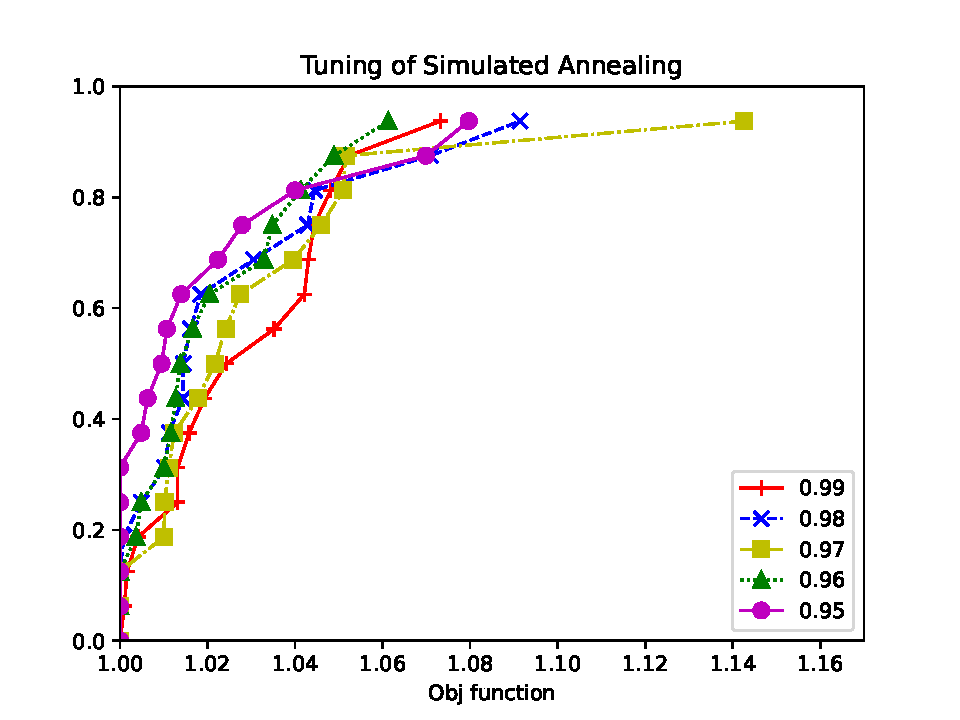
\includegraphics[width=\textwidth]{images/sa.pdf}
    \caption{Tuning of Simulated Annealing}
    \label{fig:sa}
\end{figure}